\ifdefined\standalone 
\documentclass[12pt]{article}
\usepackage{graphicx}
\usepackage{float}
\usepackage[a4paper, margin=1in]{geometry}
\usepackage[utf8]{inputenc}
\usepackage{amsmath}
\usepackage{booktabs}
\usepackage{tikz}
\usetikzlibrary{decorations.pathmorphing}
\usepackage[hidelinks]{hyperref} % <- hypertext
\usepackage{textcomp}  % <-- for \textdegree

\begin{document}
\fi

\section{Thermal equilibrium in a heterogeneous 3D block}

This verification case evaluates the ability of the thermal solver to conserve energy in a closed system.  
A cubic domain of $V_{tot}=20\times 20\times 0.20~\mathrm{cm}$ is divided into two regions:  
a hot sub‐cube of $10~\mathrm{cm}$ side located at one corner, with an initial temperature $T_\mathrm{hot} = 600^\circ\mathrm{C}$, and the remaining volume at $T_\mathrm{cold} = 20^\circ\mathrm{C}$ as shown in Figure~\ref{fig:3d_config}.  
The two regions have distinct thermophysical properties, given in Table~\ref{tab:phys_props}.  
All boundaries are adiabatic, ensuring no external heat exchange.  
The material is anisotropic to increase complexity.  
The theoretical equilibrium temperature $T_\mathrm{eq}$ is obtained from total energy conservation:
\begin{align}
H_\mathrm{hot} &= \rho_\mathrm{hot} c_{p,\mathrm{hot}} V_\mathrm{hot} T_\mathrm{hot} \; ; \;
H_\mathrm{cold} = \rho_\mathrm{cold} c_{p,\mathrm{cold}} V_\mathrm{cold} T_\mathrm{cold} \; ; \;
H_\mathrm{total} = H_\mathrm{hot} + H_\mathrm{cold}
\end{align}
\begin{equation}
T_\mathrm{eq} = \frac{H_\mathrm{total}}{\rho_\mathrm{hot} c_{p,\mathrm{hot}} V_\mathrm{hot} + \rho_\mathrm{cold} c_{p,\mathrm{cold}} V_\mathrm{cold}} \approx 116.45^\circ\mathrm{C}
\end{equation}

The time–temperature evolution at three points of the domain is shown in Figure~\ref{fig:temp_points}, and Figure~\ref{fig:slice_temp} shows a slice view at $x=5$~cm at different time steps.  
The effect of anisotropic conductivity is visible, as the heat propagation rate is higher in one direction.
\begin{table}[H]
\centering
\caption{Thermophysical properties of the two regions.}
\label{tab:phys_props}
\footnotesize
\begin{tabular}{@{}lcccccc@{}}
\toprule
Region & $T_{\mathrm{ini}}$ ($^\circ$C) &
$k_x$ &
$k_y$ &
$k_z$ ($\mathrm{W \cdot m^{-1} \cdot K^{-1}}$) &
$c_p$ ($\mathrm{J \cdot kg^{-1} \cdot K^{-1}}$) &
$\rho$ ($\mathrm{kg \cdot m^{-3}}$) \\
\midrule
Hot  & 400 & 8 & 5 & 10 & 1000 & 1000 \\
Cold & 20  & 8 & 5 & 10 & 700  & 600 \\
\bottomrule
\end{tabular}
\end{table}

\begin{figure}[H]
\centering
\begin{minipage}[t]{0.48\textwidth}
\centering
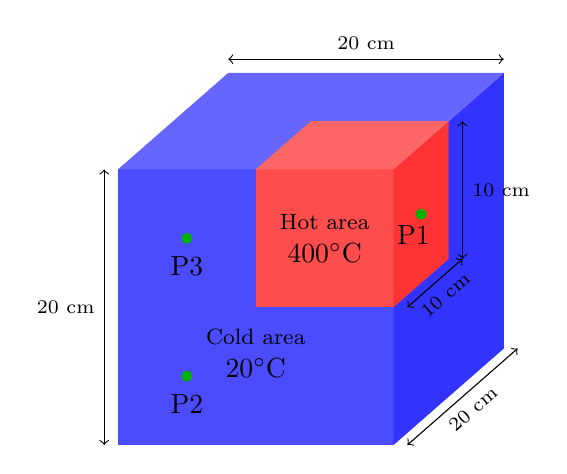
\begin{tikzpicture}[scale=1, x={(1cm,0cm)}, y={(0cm,1cm)}, z={(0.4cm, 0.35cm)}]

% Dimensions of Material A
\def\LC{3.5}  % length (x)
\def\WC{3.5}  % width  (y)
\def\HC{3.5}  % height (z)

% Cold Block
\fill[blue!70] (0,0,0) -- (\LC,0,0) -- (\LC,\WC,0) -- (0,\WC,0) -- cycle;
\fill[blue!80] (\LC,0,0) -- (\LC,\WC,0) -- (\LC,\WC,\HC) -- (\LC,0,\HC) -- cycle;
\fill[blue!60] (0,\WC,0) -- (\LC,\WC,0) -- (\LC,\WC,\HC) -- (0,\WC,\HC) -- cycle;

% Hot Block 
\def\LH{0.5*\LC}
\def\WH{0.5*\WC}
\def\HH{0.5*\HC}

\fill[red!70] (\LH,\WC-\LH,0) -- (\LC,\WC-\LH,0) -- (\LC,\WC,0) -- (\LH,\WC,0) -- cycle;
\fill[red!80] (\LC,\WC-\LH,0) -- (\LC,\WC,0) -- (\LC,\WC,\HH) -- (\LC,\WC-\LH,\HH) -- cycle;
\fill[red!60] (\LH,\WC,0) -- (\LC,\WC,0) -- (\LC,\WC,\HH) -- (\LH,\WC,\HH) -- cycle;

% Labels
\node[align=center] at (\LC -\LH/2,\WC-\WH/2,0.) {\footnotesize Hot area\\$400^\circ\mathrm{C}$};
\node[align=center] at (\LC/2,\WC/3,0) {\footnotesize Cold area\\$20^\circ\mathrm{C}$};

% Annotations
\draw[<->] (1.05*\LC,0.0*\WC,0) -- (1.05*\LC,0.0*\WC,\HC)
 node[midway, sloped, below] {\scriptsize 20~cm};

\draw[<->] (-0.05*\LC,0,0) -- (-0.05*\LC,\WC,0)
 node[midway,  align=center, anchor=east] {\scriptsize 20~cm};

\draw[<->] (0,1.05*\WC,\HC) -- (\LC,1.05*\WC,\HC)
 node[midway, sloped, above] {\scriptsize 20~cm};

\draw[<->] (1.05*\LC,\WC-\WH,\HH) -- (1.05*\LC,\WC,\HH)
 node[midway, align=center, anchor=west] {\scriptsize 10~cm};

\draw[<->] (1.05*\LC,\WH,0) -- (1.05*\LC,\WH,\HH)
 node[midway, sloped, below] {\scriptsize 10~cm};

% Point P1
\fill[green!70!black] (1*\LC,0.75*\WC,0.25*\HC) circle (2pt);
\node[black] at (1*\LC,0.7*\WC,0.18*\HC) {P1};

% Point P2
\fill[green!70!black] (0.25*\LC,0.25*\WC,0) circle (2pt);
\node[black] at (0.25*\LC,0.15*\WC,0){P2};


% Point P3
\fill[green!70!black] (0.25*\LC,0.75*\WC,0) circle (2pt);
\node[black] at (0.25*\LC,0.65*\WC,0){P3};



\end{tikzpicture}
\caption{Domain configuration}
\label{fig:3d_config}
\end{minipage}
\hfill
\begin{minipage}[t]{0.48\textwidth}
\centering
\includegraphics[width=\linewidth]{point_temperature_3D_Teq.png} 
\caption{Temperature evolution.}
\label{fig:temp_points}
\end{minipage}
\end{figure}

\begin{figure}[H]
\centering
\includegraphics[width=\linewidth]{slice_temperature_3D_Teq.png} 
\caption{Temperature distribution on the $x=5$~cm slice at different time steps.}
\label{fig:slice_temp}
\end{figure}

\ifdefined\standalone
\end{document}
\fi




